\documentclass[11pt, a4paper]{article}
%\usepackage{proj1}
\usepackage{natbib}
\usepackage{fancyhdr}  
\usepackage{subcaption}
\usepackage{caption}
\usepackage{graphicx}
\usepackage{numprint}
\usepackage{multirow}
\linespread{1.25} 
\setlength{\parindent}{0cm}
\graphicspath{{Images/}}
\usepackage{hyperref}
\usepackage{amsmath}
\usepackage{amsfonts}
\usepackage{amssymb}
\usepackage{amsthm}
\usepackage{mathtools}
\usepackage{commath}
\usepackage{bbm}
\usepackage[ruled,vlined]{algorithm2e}

%\usepackage[sc,osf]{mathpazo}
\usepackage{subcaption}
\usepackage[a4paper, top=1in, left=1.0in, right=1.0in, bottom=1in, includehead, includefoot]{geometry} %Usually have top as 1in

\usepackage{listings}
\usepackage{color} %red, green, blue, yellow, cyan, magenta, black, white
\definecolor{mygreen}{RGB}{28,172,0} % color values Red, Green, Blue
\definecolor{mylilas}{RGB}{170,55,241}


\hypersetup{colorlinks,linkcolor={black},citecolor={blue},urlcolor={black}}
\usepackage{color}
\urlstyle{same}


\theoremstyle{definition}
\newtheorem{definition}{Definition}[section]

\newcommand{\adja}{q_a}
\newcommand{\adjb}{q_b}
\newcommand{\adjaB}{q_{a,\partial \Omega}}
\newcommand{\adjbB}{q_{b,\partial \Omega}}
\newcommand{\adjB}{q_{\partial \Omega}}
\newcommand{\Adja}{\mathbf{p}}
\newcommand{\Adjb}{q}
\newcommand{\adj}{q}
\newcommand{\Adjc}{{q}_{\partial \Omega}}
\newcommand{\ra}{\rho_a}
\newcommand{\rb}{\rho_b}
\newcommand{\w}{\mathbf{w}}
\newcommand{\f}{\mathbf{f}}
\newcommand{\ve}{\mathbf{v}}
\newcommand{\n}{\mathbf{n}}
\newcommand{\h}{\mathbf{h}}
\newcommand{\K}{\mathbf{K}}
\newcommand{\hr}{\widehat \rho}
\newcommand{\jf}{\mathbf j}

\DeclareMathOperator{\sgn}{sgn}
\DeclareMathOperator{\Grad}{Grad}
\DeclareMathOperator{\Div}{Div}
\DeclareMathOperator{\Lap}{Lap}
%	\begin{figure}[h]
%		\centering
%		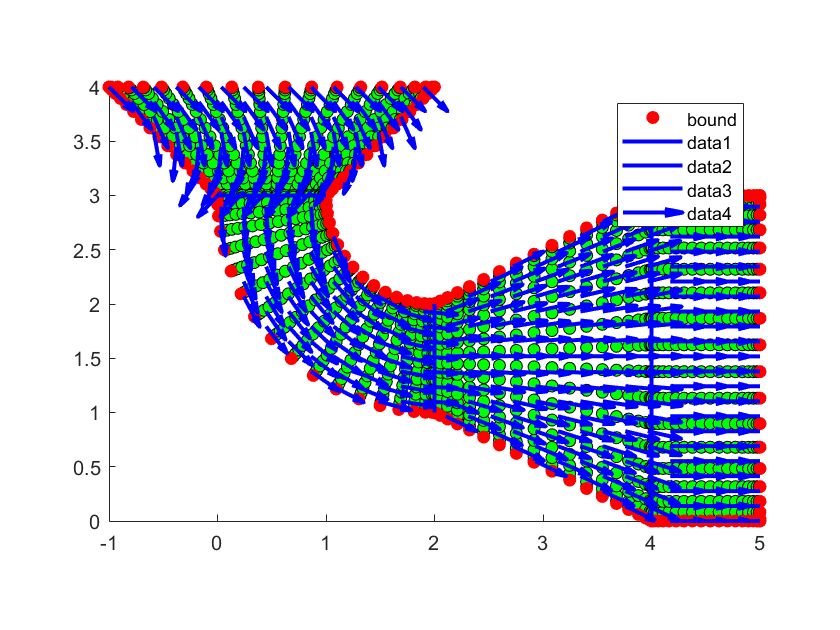
\includegraphics[scale=0.35]{F1.png}
%		\caption{Forward $\rho$ for $a = 0.01$} 
%		\label{F1}
%	\end{figure}

\begin{document}
\section{Implementation for different shapes}	
\subsection{An interval in one dimension}
\subsubsection{Discretization points, boundaries, normals}
Pseudospectral methods on non-periodic domains are based on polynomial interpolation on non-equispaced points.  
Typically, Chebyshev points $\{x_j\}$, $j = 0,..,N$, are chosen as collocation points on $[-1,1]$, which are defined as:
\begin{align}\label{defChebyshevPoints}
	x_j= \cos\bigg(\frac{j \pi}{N}\bigg), \quad j=0,1,...,N,
\end{align}	
see \cite{bibTrefethen}.
These points are clustered at the endpoints of the interval, and sparse around $0$. Using this approach, the points are distributed from $1$ to $-1$, which is counter-intuitive. Therefore, in the code library 2DChebClass \cite{GoddardPseudospectralCode1}, which is used in producing the results of this report, the Chebyshev points are automatically flipped back to run from $-1$ to $1$. All computations in 2DChebClass are done on this computational domain $[-1,1]$. A vector $\vec x$ on $[-1,1]$ can then be mapped onto a physical domain $[a,b]$ of interest via the following linear map
\begin{align}\label{eq:linearmap}
\vec y = a + \frac{(\vec x+1)(b-a)}{2}.  
\end{align}
The inverse map is 
\begin{align}\label{eq:invlinearmap}
\vec x = -1 + \frac{2(\vec y-a)}{b-a}.
\end{align}
\\
The boundary of the domain is found by creating a vector of size $N$, which contains ones at the boundary points (i.e. $x_{min}$ and $x_{max}$) and zeros everywhere else. Note that the boundary points are found by evaluating the computational minimum and maximum.
The normal vectors for the line are simply defined as the one dimensional outward normals $n_1 = -1$, located at $y_{min}$ and $n_2 = 1$ at $y_{max}$. 
\subsubsection{Interpolation}
The function of interest, $f$, is evaluated at the Chebyshev points $\{x_j\}$ and a grid function, $f_j := f(x_j)$, is defined. There exists a unique polynomial of degree $\leq N$ that can be used to interpolate a function $f$ on the grid points $x_j$. The polynomial $p_N$ satisfies, by definition, the following relationship
\begin{align}\label{eqnptov1}
	p_N(x_j)=f_j,
\end{align}
so that the residual $p_N(x_j) -f_j$ is zero at these points. Therefore, this method is called a collocation method, see \cite{Boyd1}. Interpolation on the Chebyshev grid is done using barycentric Lagrange interpolation, derived in \cite{bibTrefethenBerrut1}. The barycentric formula is
\begin{align*}
	p_N(x)= \frac{\displaystyle \sum_{k=0}^N \frac{\tilde w_j}{x-x_j}f(x_j)}{\displaystyle \sum_{j=0}^N \frac{\tilde w_j}{x-x_j}},
\end{align*}
where the weights are defined as
\begin{align*}
	\tilde w_j = (-1)^j d_j, \quad d_j = 
	\left \{
	\begin{tabular}{c}
		$\frac{1}{2}$ \text{for} $j=0$, $j=N$, \\
		$1$ \text{otherwise}, \phantom{abksla} 
	\end{tabular}
	\right .
\end{align*}
see \cite{bibTrefethenBerrut1} and \cite{GoddardPseudospectralCode1}. In the code library 2DChebClass, this is implemented as a matrix-vector product, interpolating from the set of points $\{x_j\}$, onto another set of points $\{x_i\}$, where $i = 0,...., M$ and $j = 0, ...., N$.  The interpolation matrix is of the form
\begin{align*}
	\text{Interp}_{ij} = \frac{1}{\omega_i} \left(\frac{\tilde w_j}{x_i-x_j}\right), \qquad \omega_i = \displaystyle \sum_{k=0}^N \frac{\tilde w_k}{x_i-x_k}.
\end{align*} 
Generally, the set $\{x_j\}$ lies in computational space $[-1,1]$, while the second set of points can be customised by the user, to be any $M$ points in $[a,b]$. There is another function in 2DChebClass, which takes a set of $N$ points $\{x_j\}$ in physical space as the input. This set of points is then first mapped onto the computational domain, using a linear map, before the interpolation matrix is computed, as described above. This method can then be applied to interpolating an arbitrary set of values $\{f_j\}$ onto the new set of points $\{f_i\}$. 
\subsubsection{Differentiation}
The derivation of the Chebyshev differentiation matrices is described below, following the presentation in \cite{bibTrefethen}. Given a polynomial $p_N$ (++definitely same as above??++), where condition \eqref{eqnptov1} holds, it can be differentiated so that $f'_j = p'(x_j)$, which can be rewritten as a multiplication of $f_j$ by a $(N+1) \times (N+1)$ matrix, denoted by $D$, as follows
\begin{align*}
	f'_j= D f_j,
\end{align*}
using (\ref{eqnptov1}).
A $(N+1) \times (N+1)$ differentiation matrix $D$ has the following entries, compare with \cite{bibTrefethen}
\begin{align*}
	(D)_{00}&= \frac{2N^2 +1}{6},\\
	(D)_{NN}&= -\frac{2N^2 +1}{6},\\
	(D)_{jj}&= -\frac{x_j}{2(1-x_j^2)}, \quad j=1,...,N-1,\\
	(D)_{ij}&= \frac{c_i}{c_j} \frac{(-1)^{i+j}}{(x_i-x_j)}, \quad i \neq j, \quad i,j=0,...,N,
\end{align*} 	
where 
\begin{align*}
	c_i =\left\{\begin{array}{l} 2, \quad i=0 \text{   or   }N, \\1, \quad \text{otherwise.}\end{array}\right.
\end{align*}	
The second derivative is represented by the second differentiation matrix $D_2$, which can be found by squaring the first differentiation matrix; $D_2=D^2$, and more generally the $j^{th}$ differentiation matrix is found as follows
\begin{align*}
	D_j=D^j.
\end{align*}
However, in \cite{GoddardPseudospectralCode1}, the exact coefficients, derived in a similar way as above for $D$, are used to compute $D_2$, since it is more accurate than squaring $D$. Furthermore, all differentiation matrices are derived in computational space and then mapped to physical space using a Jacobian transformation. (++ details?++)
\subsubsection{Integration}
In order to evaluate integrals in a similar way, the so-called Clenshaw--Curtis quadrature is used, which is derived in \cite{ClenCurt1}.
This is, for the integral over a smooth function $f$:
\begin{align}\label{eqnClenCurtQuad}
	\int_{-1}^1 f(x)dx = \sum_{k=0}^N w_kf(x_k),
\end{align}
where the weights are defined as:
\begin{align*}
	w_j = \frac{2d_j}{N}
	\left \{
	\begin{tabular}{c}
		$1- \displaystyle \sum_{k=1}^{(N-2)/2} \frac{2 \cos(2kt_j)}{4k^2-1} - \frac{\cos(\pi j)}{N^2 -1} \quad \quad\text{for $N$ even}$,\\
		$1- \displaystyle \sum_{k=1}^{(N-2)/2} \frac{2 \cos(2kt_j)}{4k^2-1} \quad \quad \quad \quad \quad \quad \ \ \ \text{for $N$ odd}$,
	\end{tabular}
	\right .
\end{align*}
see \cite{GoddardPseudospectralCode1}. In 2DChebClass this is implemented as a vector, such that $(\text{Int})_k = w_k$. Again, this is done in computational space, so that a Jacobian transformation has to be taken to map this onto a desired physical domain. A dot product can be taken between a vector with entries $f_j$ and the resulting integration vector. 
\subsubsection{Convolution}
The final aspect to be considered is the convolution matrix, which is needed to compute convolution integrals. 
The convolution integral is defined as:
\begin{align*}
	\left(n \star \chi \right) (\vec y) = \int \chi ( \vec y - \vec{ z}) n (\vec{z}) d \vec{z}.
\end{align*}
A convolution matrix Conv can be created as follows
\begin{align*}
	\text{Conv}_{i,j} = \text{Int}_j \ \ \chi( y_i -  y_j)
\end{align*}
where $\vec y$ is the vector of physical points in $[a,b]$.
 The convolution integral is now defined as matrix vector multiplication, by applying the matrix Conv to a density vector $n$. The convolution matrix can be applied to different densities $n$, which saves computational time. 



\subsection{The quadrilateral}
\subsubsection{Discretization points and domains}
We now consider two dimensional domains with the set of points $\{X_j\} = \{(x_1^j,x_2^j)\}$, where $j = 1, ..., N$ in the computational domain $[-1,1]^2$.

In order to extend the one dimensional considerations to two-dimensional grids, a so-called tensor product grid has to be defined. First, Chebyshev points $x_1^j$, for $j=1,...,N$, on the $x$-axis and another set of Chebyshev points $x_2^i$, for $i=1,...,M$ on the $y$-axis are taken, both between $[-1,1]$. 
Then the following two so called Kronecker vectors are defined:
\begin{align}\label{eq:KroneckerVec}
	\mathbf{x}_1^{K}&=(x_1^1,x_1^1,...,x_1^1,x_1^2,x_1^2,...,x_1^2,...,x_1^n,x_1^n,...,x_1^n)^T,\\
	\mathbf{x}_2^{K}&=(x_2^1,x_2^2,...,x_2^m,x_2^1,x_2^2...,x_2^m,.....,x_2^1,x_2^2,...,x_2^m)^T.\notag
\end{align} 
In $\mathbf{x}_1^{K}$, each $x_1^j$ is repeated $m$ times, while $\mathbf{x}_2^{K}$, each sequence $x_2^1,x_2^2,...,x_2^m$ is repeated $n$ times. The total length of each vector is $n \times m$. 
These vectors are defined, so that the set $(\mathbf{x}_1^{K},\mathbf{x}_2^{K})$ is a full set of all Chebyshev points on the two-dimensional tensor grid in computational space. An equivalent set can be defined for the points on the physical domain. Note that the points are clustered around the boundary of the two-dimensional grid and sparse in the middle of the grid.
\\
\\
As in the one dimensional case we can map the points $(\mathbf{x}_1^{K},\mathbf{x}_2^{K})$ to an arbitrary quadrilateral shape discretized via $(\mathbf{y}_1^{K},\mathbf{y}_2^{K})$. We use the superscript $k$ to indicate that $x^k \in \mathbf{x}^{K}$, for $k = 1,....,n \times m$. We first apply a linear map from $[-1,1]^2$ to $[0,1]^2$ 
\begin{align*}
	x_1^k = \frac{x_1^k+1}{2}, \quad
	x_2^k = \frac{x_2^k+1}{2}.
\end{align*}
Then the bilinear maps
\begin{align}\label{eq:bilinear1}
	y_1^k &= \alpha_1 + \alpha_2 x_1^k + \alpha_3 x_2^k + \alpha_4 x_1^k x_2^k,\\
	y_2^k &= \beta_1 + \beta_2 x_1^k + \beta_3 x_2^k + \beta_4 x_1^k x_2^k. \notag
\end{align}
take the points on the computational domain to the ones on the physical domain. The $\alpha_i$, $\beta_i$ are determined by mapping the coordinates of the four corners of the computational domain in a cyclic order onto the corners of the quadrilateral. 
The Jacobian of this bilinear map is also saved in this step, as well as the Hessians with respect to both variables.
However, most of the time we are given the coordinates of the quadrilateral in physical space, so that we have to map back to the computational domain. In order to do this, we again need to first find the values of the parameters $\alpha_i$ and $\beta_i$ and then invert the bilinear map to solve for the set of points on the computational domain.
We define a matrix B, with $A = BY$, such that $A_i = (\alpha_i, \beta_i)$, where $i = 1,2,3,4$, based on the bilinear maps \eqref{eq:bilinear1}, as
\begin{align*}
	B  =
	\begin{pmatrix}
		1 & 0 & 0 & 0 \\
		- 1 & 1 & 0 & 0 \\
		-1 & 0 & 0 & 1 \\
		1 & -1 & 1 & -1
	\end{pmatrix}	.
\end{align*}
Once we know the values of the parameters, we can solve the inverse map
\begin{align*}
	x_1^k = \frac{y_1 - \alpha_1 -\alpha_3 x_2^k}{\alpha_2 + \alpha_4 x_2^k}
\end{align*}
and the quadratic
\begin{align*}
	a&\left(x_2^k\right)^2 + bx + c = 0,\\
	a &= \alpha_4 \beta_3 - \alpha_3 \beta_4,\\
	b &= \alpha_4 \beta_1 - \alpha_1 \beta-4 + \alpha_2 \beta_3 -\alpha_3 \beta_2 + y_1^k \beta_4 - y_2^k \alpha_2,\\
	c &= \alpha_2 \beta_1 - \alpha_1 \beta_2 + y_1^k \beta_2 - y_2^k \alpha_2.
\end{align*}
These give us the values for the $x_1^k$ and $x_2^k$ on $[0,1]^2$. In order to map to the computational domain $[-1,1]^2$, we apply a final linear map
\begin{align*}
	x_1^k = 2x_1^k - 1 \quad	x_2^k = 2x_2^k - 1.
\end{align*}


\subsubsection{Boundaries and Normals}
We can define the boundary of the quadrilateral by defining vectors for each of the four sides of the quadrilateral as follows. We do this on the computational domain $[-1,1]^2$, since each of the sides of the computational domain is conformally mapped onto a corresponding side of the quadrilateral. It is then straightforward to define a boolean vector of size $n \times m$, which contains ones where $x_1 == x_{1,min}$ and zeros everywhere else, to define the left boundary of the square. We can then do the same for the other sides. We combine these four vectors to one boundary vector, which contains ones at each of the four faces and zeros everywhere else. (++ edit and make clearer. Maybe write out some of this ++)
\\
The normal vectors of the quadrilateral are found by considering the four corners of the shape. We have the four corners $\{Y_i\} = \{(y_1^i,y_2^i)\}$, starting from the left bottom corner and defined in clockwise order. We then have the following set of normals $n_l$, $n_r$, $n_t$, and $n_b$, for the left, right, top and bottom normal respectively.
For the left normal we first define the vector
\begin{align*}
     \vec m_l = \left(y_2^2 - y_2^1, y_1^2 - y_1^1 \right) := \left(m_{l,1},m_{l,2} \right). 
\end{align*}
We then define the normal to be
\begin{align*}
	\vec n_l =  \sgn (m_{l,1})\frac{\left(-m_{l,1},m_{l,2} \right)}{\sqrt{m_{l,1}^2+m_{l,2}^2 }},
\end{align*}
where the negative first component and $\sgn (m_{l,1})$ are taken so that we 
consider the outward normal. We furthermore want to work with the unit normal, which is the reason for the normalisation term. The other three normals are therefore defined as
\begin{align*}
	\vec n_r &=  \sgn (m_{r,1})\frac{\left(m_{r,1}, - m_{r,2} \right)}{||\vec m_{r} ||_{l_2}},\\
	\vec n_t &=  \sgn (m_{t,2})\frac{\left(-m_{t,1},m_{t,2} \right)}{||\vec m_{t} ||_{l_2}},\\
	\vec n_b &=  \sgn (m_{b,2})\frac{\left(m_{b,1},-m_{b,2} \right)}{||\vec m_{b} ||_{l_2}}.
\end{align*}
In each of these terms, the definition of the $m_1$ is the difference in $y_2$ components, where the top coordinate is subtracted from the bottom coordinate and the $m_2$ refer to the left $y_1$ value being subtracted from the right $y_1$ value.
Each of these normal vectors has values on its respective face of the quadrilateral and zeros everywhere else. We then combine these four vectors using the boundary boolean vector which we have defined in the above step. This means that the normals on the corners get summed together, since each of the two faces meeting at a corner has a normal defined at the corner. This normal at a corner is not uniquely defined. However, it is convenient to define it such that it is the average of the two normals from each shape. This is done by normalising the sum of the two added normals, as demonstrated here for the corner normal between the left and top face of the quadrilateral
\begin{align*}
	\vec n_c = \frac{\left(\vec n_{l} + \vec n_{t} \right)}{||\vec n_{l} + \vec n_{t}  ||_{l_2}}.
\end{align*}

\subsubsection{Interpolation}
Interpolation in two dimensions is based on the idea of Kronecker tensor products. The interpolation matrices $\text{Interp}_1$ and $\text{Interp}_2$ are computed for both sets of points $\{x_1^j\}$ on the $x$-axis and $\{x_2^i\}$ in the $y$ direction. The Kronecker product of these two matrices is taken resulting in the two-dimensional interpolation matrix. For an example with $i = j = 1,2,3$, this is the block matrix of size $ 9 \times 9$
\begin{align*}
	\text{Interp} &= \text{Interp}_1 \otimes \text{Interp}_2 \\
	&= 
	\begin{pmatrix}
		\text{Interp}_1(1,1) \times \text{Interp}_2 & \text{Interp}_1(1,2) \times \text{Interp}_2& \text{Interp}_1(1,3)  \times \text{Interp}_2\\
		\text{Interp}_1(2,1)  \times \text{Interp}_2 & \text{Interp}_1(2,2) \times  \text{Interp}_2& \text{Interp}_1(2,3)  \times \text{Interp}_2\\
		\text{Interp}_1(3,1)  \times \text{Interp}_2 & \text{Interp}_1(3,2)  \times \text{Interp}_2& \text{Interp}_1(3,3)  \times \text{Interp}_2
	\end{pmatrix}.
\end{align*}
\subsubsection{Differentiation}
A similar approach, using Kronecker vectors, can be used to find the Chebyshev differentiation matrices for two-dimensional problems as follows, compare to \cite{bibTrefethen}. For a first derivative $D$ in the $x$ direction, a Kronecker product is taken of the one-dimensional Chebyshev differentiation matrix with the identity, as demonstrated here with three points
\begin{align*}
	D_{x_1}&=I \otimes D = 
	\begin{pmatrix}
		1 & 0 & 0\\
		0 & 1 & 0 \\
		0 & 0 & 1
	\end{pmatrix}
	\otimes
	\begin{pmatrix}
		d_{11} & d_{12} & d_{13}\\
		d_{21} & d_{22} & d_{23} \\
		d_{31} & d_{32} & d_{33}
	\end{pmatrix}
	\\&=
	\begin{pmatrix}
		d_{11} & d_{12} & d_{13} & & &  & & &\\
		d_{21} & d_{22} & d_{23} & & & & & & \\
		d_{31} & d_{32} & d_{33} & & & & & & \\
		& & &d_{11} & d_{12} & d_{13} & & &\\
		& & &d_{21} & d_{22} & d_{23}  & & &\\
		& & &d_{31} & d_{32} & d_{33} & & &\\
		& & & & & &d_{11} & d_{12} & d_{13}\\
		& & & & & &d_{21} & d_{22} & d_{23}  \\
		& & & & & &d_{31} & d_{32} & d_{33} 
	\end{pmatrix},
\end{align*}
where the block structure matches the repetition of each $x_1^j$ in $\mathbf{x}_1^{K}$.
The second derivative with respect to ${x_1}$, $D_{x_1x_1}$ can be found by using $D_2$ instead of $D$ in this calculation. 
The derivative with respect to $y$ is found by taking the Kronecker product the other way around
\begin{align*}
	D_{x_2}&=D \otimes I = 
	\begin{pmatrix}
		d_{11} & d_{12} & d_{13}\\
		d_{21} & d_{22} & d_{23} \\
		d_{31} & d_{32} & d_{33}
	\end{pmatrix}
	\otimes
	\begin{pmatrix}
		1 & 0 & 0\\
		0 & 1 & 0 \\
		0 & 0 & 1
	\end{pmatrix}
	\\&=
	\begin{pmatrix}
		d_{11} & & & d_{12} & & & d_{13} & & \\
		& d_{11} & & & d_{12} & & &  d_{13} & \\
		& & d_{11} & & &  d_{12} &  & & d_{13}\\
		d_{21} & & & d_{22} & & & d_{23} & & \\
		& d_{21} & & & d_{22} & & &  d_{23} & \\
		& & d_{21} & & &  d_{22} &  & & d_{23}\\
		d_{31} & & & d_{32} & & & d_{33} & & \\
		& d_{31} & & & d_{32} & & &  d_{33} & \\
		& & d_{31} & & &  d_{32} &  & & d_{33}\\
	\end{pmatrix},
\end{align*}
which now matches the repetition of each $x_2^1,...x_2^m$ in $\mathbf{x}_2^{K}$.
All of the two dimensional differentiation matrices are computed in computational space $[-1,1]^2$, and therefore need to be mapped to the physical domain. This is done by premultiplying by the inverse transpose of the Jacobian of the transformation between the physical and computational space. We get the differentiation matrices in physical space $D_{y_1}$ and $D_{y_2}$. The same can be done for the second derivative, using the Hessian matrices for $y_1$ and $y_2$.
We have the following operators for the quadrilaterals
\begin{align*}
	\Grad &= \left(D_{y_1}, D_{y_2}\right),\\
	\Div &=\left(D_{y_1}, D_{y_2}\right)^\top,\\
	\Lap &= D_{y_1y_1} + D_{y_2y_2}.
\end{align*}

\subsubsection{Integration}
The two dimensional integration vector is found by considering the two integration vectors for the points in the $x$ and the $y$ axis directions. The Kronecker product of these are taken and then multiplied by the determinant of the Jacobian of the mapping to the physical domain, since the integration vectors are computed on the computational grid. This gives the two dimensional integration vector.

\subsubsection{Convolution}
The construction of the convolution matrix is identical to the one in the one dimensional case, except that $\chi$ takes both $\mathbf{y}_1^{K}$ and $\mathbf{y}_2^{K}$ as inputs and the integration vector involved is the two dimensional integration vector.
We have
\begin{align*}
	\text{Conv}_{i,j} = \text{Int}_j \ \ \chi({y}_1^{i} - {y}_1^{j},{y}_2^{i} - {y}_2^{j}).
\end{align*}
If the function $\chi$ only takes one input, we  consider the two given differences of points 
\begin{align*}
	d_1^{i,j} = {y}_1^{i} - {y}_1^{j}, \quad
	d_2^{i,j} = {y}_2^{i} - {y}_2^{j},
\end{align*}
and compute the euclidean distance between $d_1$ and $d_2$ to get the convolution matrix
\begin{align*}
	\text{Conv}_{i,j} = \text{Int}_j \ \ \chi(||d_1^{i,j}, d_2^{i,j}||_{l_2}).
\end{align*}

\subsection{The wedge}
\subsubsection{Domains, boundaries, normals}
A wedge is a section of an annulus, the boundary of which is defined by an inner and outer radius $r$ as well as a minimum and maximum angle $\theta_1$ and $\theta_2$. While $\theta_1$ should be chosen to lie in $[0, 2 \pi]$, the coordinate $\theta_2$ is mapped into this principal domain by computing 
\begin{align*}
	\theta_2 = \theta_1 +  d, \quad \text{where} \quad d = \theta_2 - \theta_1\mod 2 \pi.
\end{align*}
The wedge can be conformally mapped to a computational domain $[-1,1]^2$ (in polar coordinates ?!). For this the Kronecker vectors \eqref{eq:KroneckerVec} for the computational points $\{x_1\}$ and $\{x_2\}$ are taken. 
The Kronecker points $\mathbf{x}_1^{K}$ and $\mathbf{y}_1^{K}$ can then be mapped to the physical domain in $r$ and $\theta$ using the linear map \eqref{eq:linearmap} and then back to the computational domain using the map \eqref{eq:invlinearmap} from the one dimensional code. The derivatives of the map \eqref{eq:linearmap} for both variables are stored in the Jacobian matrix $J$.
\\
\\
The boundaries of this shape are found in an identical manner to the quadrilateral case, since this is based on the computational grid. The definition of the normals in polar coordinates is straightforward, since this can be thought of as a square (++ explain better ++). On the side with $\theta = \theta_2$ and on $r = r_2$ we have that $\vec n = (1,0)$, $\vec n = (0,1)$ and on the boundaries where $\theta = \theta_1$ and on $r = r_1$, we get that $\vec n = (-1,0)$, $\vec n = (0,-1)$. Since these are added together to result in the full set of normals, the set of normals at the corners is $\{\vec n_c\} = \{(-1,-1), (-1,1), (1,-1), (1,1)\}$. 


\subsubsection{Interpolation and differentiation}
Since interpolation is done on the computational grid (++ check ++) this does not change from the quadrilateral case.
\\
\\
In order to derive the differentiation matrices for the wedge, we start with the one-dimensional differentiation matrices described in the previous section. Since these are derived on the computational domain, we have to map them to the physical domain. This is done for each coordinate individually so that we have
\begin{align*}
	D_r = J_1D \otimes I \quad 	D_\theta =I \otimes J_2D,
\end{align*} 
where $D$ is the differentiation matrix for the one-dimensional domain and $J_1$ and $J_2$  are the corresponding Jacobians of the mapping from the computational to the physical domain. For each discretization point $j = 1,...,N$ we have $ J_1^j= \frac{dr^j}{dx_1^j}$ and $J_2^j = \frac{d\theta^j}{dx_2^j}$.
However, this will result in differentiation matrices with respect to the coordinates $r$ and $\theta$. In order to compute the gradient, divergence and Laplacian we have to use the standard definition of the polar versions to derive these. For $ r \neq 0$ we get
\begin{align*}
	\Grad  &= \left(D_r, \frac{1}{r} D_\theta\right) ,\\
	\Div &= \left(D_r + \frac{1}{r}, \frac{1}{r} D_\theta\right)^\top ,\\
	\Lap  &= D_{rr} +\frac{1}{r}D_r +  \frac{1}{r^2} D_{\theta \theta}.
\end{align*}
At $ r = 0$, we need to treat these operators more carefully. We know that $\frac{1}{r} D_\theta = D_{r\theta}$, since $D_\theta =0$ at $r = 0$, and so $ \Grad = \left(D_r, D_{r\theta}\right)$. Similarly, at $r = 0$, we get that $\Div = \left(2D_r, D_{r\theta}\right)^\top$. Finally we have that $\Lap = 2 D_{rr} + \frac{1}{2} D_{\theta\theta}D_{rr}$ at the origin. (++ go back and think why ++)


\subsubsection{Integration and convolution}
The integration vector is found in the same way as done for the quadrilateral. However, since this is an integral in polar coordinates, in a last step the integration vector has to be multiplied pointwise by $r$ to satisfy the polar integration formula $\int \int f(r, \theta) r dr d\theta$.
\\
\\
The convolution matrix is computed in the same way as for the quadrilateral, now using the polar version of the integration vector.

\subsection{The periodic box}
\subsubsection{Domains, boundaries, normals}
The periodic box has the first coordinate in in Cartesian space, discretized with Chebyshev points, the second coordinate is in Fourier space, using an equispaced discretization. This coordinate $\vec x_2$ is periodic. 
This means that while for the first coordinate $\vec x_1$ the linear maps \eqref{eq:linearmap} and \eqref{eq:invlinearmap} are still used, for the second coordinate we have the map 
\begin{align*}
	\vec y = a + (b-a) \vec x, 
\end{align*}
from $[-1,1]$ to $[a,b]$ and the corresponding inverse map
\begin{align*}
   \vec x = \frac{\vec y- a}{b-a}.
\end{align*}
The Kronecker vectors are created in the same way as in the case for the wedge.
\\
The boundary is defined from the computational domain, as in the previous shapes. The normals are defined equivalently to the ones in the wedge, since the periodic box only has the unit normals.

\subsubsection{Interpolation}
In order to construct the interpolation matrix for this problem, we need to consider the interpolation matrices for each coordinate and take the Kronecker product of them.
The interpolation matrix for $\vec x_1$ is constructed following the description for one-dimensional domains, using barycentric Lagrange interpolation.
However, the interpolation matrix for $\vec x_2$ is constructed using discrete Fourier Transforms. The account below follows the work in \cite{bibTrefethen}.
The DFT formula is
\begin{align*}
	\hat v_k = h \sum_{j = 1}^{N} e^{-ikx_j} v_j, \quad k = - \frac{N}{2} + 1, ..., \frac{N}{2},
\end{align*}
with stepsize $h$, and the inverse transform is
\begin{align*}
	v_j = \frac{1}{2 \pi} \sum_{k = - N/2 +1}^{N/2} e^{i k x_j} \hat v_k, \quad j = 1, ..., N.
\end{align*}
This inverse transform is well equipped to act as an interpolant for polar functions on periodic grids with period $2\pi$, once a small adjustment is made. We need to define $\hat v_{-N/2} = \hat v_{N/2}$ and get the interpolant
\begin{align*}
	p(x) = \frac{1}{4 \pi} e^{- i N x/2} \hat v_{-N/2} + \frac{1}{4 \pi} e^{i N x/2} \hat v_{N/2} + \frac{1}{2 \pi} \sum_{k = - N/2 + 1}^{N/2 - 1} e^{i k x} \hat v_k, \quad j = 1, ..., N,
\end{align*}
where $x \in [-\pi/h, \pi/h]$, $h = 2\pi /N$.
An equivalent definition of the interpolant is derived by considering the interpolant for the delta function, see \cite{bibTrefethen} for a derivation.
We get
\begin{align*}
	p(x) = \sum_{m = 1}^N v_m S_N(x -x_m), 
\end{align*}
where
\begin{align}\label{eq:PeriodicInterpolant}
	S_N(x) = \frac{\sin(\pi x /h)}{(2 \pi /h)\tan(x/2)}
\end{align}
The interpolation matrix for the periodic variable in the code is defined as
\begin{align*}
	\text{Interp}_{2} = \left[e^{2\pi i \vec {x}_2^{I} 0}, e^{2\pi i \vec {x}_2^{I} j_1}, \cos(2\pi i \vec {x}_2^{I} M) ,e^{2\pi i \vec {x}_2^{I} j_2}\right],
\end{align*} 
where $j_1 = 1,..., M-1$, $j_2 = M + 1,..., N$ and $M = (N + 1) /2$ if $N$ is odd and $M = N /2$ if $N$ is even. The set $\vec {x}_2^{I}$ is the set of points on which the second coordinate is interpolated on.
The fast Fourier transform matrix is defined as
\begin{align*}
	\text{FFTM} = I \otimes F, \quad \text{where} \quad	\text{F}_{jk} =  e^{- 2 \pi i / N jk},
\end{align*}
where $j, k = 0,..., N -1$.
The interpolation matrix is then
\begin{align*}
	\text{Interp} = \Re\left(\left(\text{Interp}_{1} \otimes \text{Interp}_{2}\right) \text{FFTM}\right).
\end{align*}


\subsubsection{Differentiation}
In order to derive the differentiation matrices for the periodic grid, we return to the periodic interpolant \eqref{eq:PeriodicInterpolant}. This can be differentiated to give 
\begin{align*}
	S'_N(x_j) =\left\{\begin{array}{l} 0, \phantom{(-1)^j \cot(j h /2)} \quad j \equiv 0  \mod N\\
	\frac{1}{2} (-1)^j \cot(j h /2), \quad j \not \equiv 0  \mod N.\end{array}\right.
\end{align*}
This gives one column of the differentiation matrix, which has Toeplitz structure and is created in the code as, see \cite{bibTrefethen}
\begin{align*}
	D_{x_2} = 2\pi
	\begin{pmatrix}
		0 & & &  & &  & &-\frac{1}{2} \cot(h /2) \\
		-\frac{1}{2} \cot(h /2)&  & & &  & &   &\frac{1}{2} \cot(h) \\
		\frac{1}{2} \cot(h)& &  & & &    & & -\frac{1}{2} \cot(3 h /2)\\
		-\frac{1}{2} \cot( 3 h /2) & & &   & &  & & \\
		&  & & &   & &  & \\
		& & & &  & & & \frac{1}{2} \cot(h /2)\\
		\frac{1}{2} \cot(h /2)& &  & &   &  & & 0\\
	\end{pmatrix}.
\end{align*}
The factor of $2\pi$ is there to map the matrix back onto the grid $[-1,1]$. 
For the first coordinate $x_1$, the differentiation matrix is derived on the Chebyshev grid, as in the one-dimensional example. The two differentiation matrices are each mapped onto the physical domain, using Jacobian transformations and the appropriate Kronecker products are taken to create $\Grad, \div$ and $\Lap$ for the periodic box. This assembly follows the same steps as described for the quadrilateral code.


\subsubsection{Integration and convolution}
We use the Clenshaw-Curtis integration weight in the first coordinate, as done in the one dimensional case. This is multiplied by the one-dimensional Jacobian to map these weights from the computational onto the physical domain. In the fourier domain however, the integration weights are just $1/N$. These are also multiplied by the corresponding one-dimensional Jacobian. The integration vector is then the Kronecker product of the two integration vectors.
\\
\\
The convolution matrix is constructed in the same way as for the quadrilateral. However, in the quadrilateral case we computed the function $\chi$ at $\left(\vec {y}_1^{i} - \vec {y}_1^{j}, \vec{y}_2^{i} - \vec {y}_2^{i} \right)$. In the periodic box however, we need to consider the distances of ${y}_1^{i} - {y}_1^{j}$ and ${y}_2^{i} - {y}_2^{j}$, and compute them in two different ways. 
For the Chebyshev coordinate, nothing changes and we set $d_1^{i,j} = {y}_1^{i} - {y}_1^{j}$. For the periodic variable however, we need to compute 
\begin{align*}	
	d_2^{i,j} = c^{i,j} - \frac{L}{2}, \quad \text{where} \quad c^{i,j} =  {y}_2^{i} - {y}_2^{j} + \frac{L}{2} \mod L,
\end{align*}
where $L = y_2^{max} - y_2^{min}$. 
Then convolution matrix is
\begin{align*}
	\text{Conv}_{i,j} = \text{Int}_j \ \ \chi(d_1^{i,j}, d_2^{i,j}),
\end{align*}
where $\text{Int}$ is the integration matrix for the periodic box.
If the function $\chi$ only takes one input, we take the euclidean distance between $d_1$ and $d_2$ and compute
\begin{align*}
	\text{Conv}_{i,j} = \text{Int}_j \ \ \chi(||d_1^{i,j}, d_2^{i,j}||_{l_2})
\end{align*}


\section{Convergence Stuff}
+++++++++++++++ More on convergence stuff... see Boyd +++++++++++++++++++++++
The advantage of Spectral Methods is that, for smooth functions, the convergence is exponential, see \cite{Boyd1}:
\begin{align*}
	\text{Pseudospectral Error} \approxeq O \bigg[ \bigg( \frac{1}{N} \bigg)^N \bigg].
\end{align*}


A good overview on spectral methods is given in \cite{bibTrefethen} and a more in depth discussion can be found in \cite{Boyd1}.


\section{Implementation for multishape}
In the previous section we have discussed the implementation of the methods for different single shapes. While 2DChebClass supports solutions to PDEs on various single shapes, the method is now extended to compute the solution to a PDE on a multishape. A multishape is a complex domain, which is not fully described by one of the single shapes introduced in the previous section. However, it is possible to discretize the multishape domain in such a way that each of the elements is either a quadrilateral or a wedge. While that does not include all possible complex shapes, such as triangles, it does describe most physically relevant domains. The philosophy of this multishape code is to use the existing code library \cite{GoddardPseudospectralCode1}, which is designed to efficiently and accurately solve PDEs on individual shapes, to do the same on a multishape with minimal additional effort for the user.
\\
\\
The solution of a PDE on such a multishape domain is achieved by employing the spectral element method (SEM), since the multishape is discretized into elements. This method is similar in spirit to the finite element method (FEM). FEM discretizes a domain into elements and computes the solution to a given PDE on each of those elements. Expansions of basis functions are used, which are low order polynomials, for interpolation on an equispaced grid. SEM follows the same philosophy but uses higher order basis functions such as Chebyshev or Lagrange polynomials and Chebyshev-Lobatto points on an interpolation grid on each element, as opposed to an equispaced grid, to avoid the Runge phenomenon. At the intersections between the elements, $C^0$ continuity is enforced. SEM was first introduced by Patera \cite{SEMPatera84} using  Chebyshev polynomials as basis functions and later adapted to Lagrange polynomials by Komatitsch and Vilotte \cite{SEMLagrange98}.
While this method is widely used to solve PDEs in their weak form, in this work the strong form of the PDE is considered, since this aligns best with the existing framework. (?!) Furthermore, instead of just requiring continuity of the solution at the intersection of two elements, the flux (or first derivatives) are also matched. 
+++ say that this is because we need two matching conditions and why -- why? +++
\\
\\
\subsection{Setting up the multishape}
In order to set up a multishape, each of the discretized elements have to be specified. The information that has to be given for each element is number of discretization points $N_1$ in the $x$-direction, $N_2$ in the $y$-direction, whether it is a quadrilateral or a wedge and whether to match the internal boundaries. For a quadrilateral, the four coordinates of the edges have do be given. For a wedge, inner and outer radius, maximum and minimum angle as well as the origin of the wedge have to be given. 
As done throughout in the code, the main idea is to stack the vectors and matrices of an individual element to result into a long vector of size $M \times 1$, where $M = \sum_i N^i_1 N^i_2$, where $i$ counts the number of elements in the multishape. This stacking results in computation being done directly on the multishape, instead of individually on each element. (++ improve explanation ++)
\\
\\
In order to create a functioning multishape, the number of points of the neighbouring faces of two elements have to match. Furthermore, it has to be specified whether the solution and flux at the boundary between two elements should be matched or whether no-flux boundary conditions should be imposed, to create a hard wall between two elements.
Once this information is given, the vectors of computational points $\mathbf x_1^M$, $\mathbf x_2^M$ and physical points $\mathbf y_1^M$, $\mathbf y_2^M$ on the whole multishape can be set up. This is done as described in Algorithm \ref{alg:msPts}.
 One important thing to notice is now that the vectors $\mathbf y_1^M$, $\mathbf y_2^M$ are now entirely in Cartesian coordinates, even if some of the underlying shapes are wedges, which use polar coordinates.

\begin{algorithm}[H]	\label{alg:msPts}
	\SetAlgoLined
	\For{shape $i$ in multishape}{
		Get computational points $\mathbf x_1^i$, $\mathbf x_2^i$\;
		Get physical points $\mathbf y_1^i$, $\mathbf y_2^i$\;
		Add to vector containing multishape points 
		\begin{align*}
		\mathbf x_1^M = [\mathbf x_1^M; \mathbf x_1^i], \quad
		\mathbf x_2^M = [\mathbf x_2^M; \mathbf x_2^i], \quad
		\mathbf y_1^M = [\mathbf y_1^M; \mathbf y_1^i], \quad
		\mathbf y_2^M = [\mathbf y_2^M; \mathbf y_2^i].
		\end{align*}
	}
\For{shape $i$ in multishape}{
	\eIf{shape $i$ is wedge}{
		Convert polar $\mathbf y_1^i$, $\mathbf y_2^i$ to cartesian points $\mathbf y_{1, \text{Cart}}^i$, $\mathbf y_{2, \text{Cart}}^i$\;
		Replace in $\mathbf y_1^M$, $\mathbf y_2^M$
		\begin{align*}
			\mathbf y_1^M(\text{ishape}) = \mathbf y_{1, \text{Cart}}^i, \quad \mathbf y	_2^M(\text{ishape}) = \mathbf y_{2, \text{Cart}}^i.
		\end{align*}
	}{continue;}
}
\caption{Multishape points}
\end{algorithm}

\subsection{Boundaries and intersections}
In order to  determine the points that lie on the boundary of a multishape, we first have to determine which faces of which shapes intersect. Once we have this information, we can take the boundaries of the individual shapes and substract the intersection boundaries from these to get the multishape boundary.
The intersections between shapes are found by the code automatically, as explained in Algorithm \ref{alg:msIntersections}. We iterate through all pairs of shapes to check whether any of their faces intersect by comparing the points of each shape on these faces. One thing to note is that we also have to check whether the points on face $i$ are equal to the flipped vector of points on face $j$. This is to account for the fact that there are different ways of constructing these points on each shape.
Having found the intersections between the shapes, the boundary of the multishape is defined by a boolean vector, as in the case for simple shapes. Algorithm \ref{alg:msBoundary} explains the steps.

\begin{algorithm}[H]
	\SetAlgoLined
	We loop through all faces of each two pairs of shapes to determine which faces intersect. 
	\For{ishape in multishape}{
		\For{jshape in multishape}{		
			\For{iface in ishape}{
				\For{jface in jshape}{
					\uIf{$Pts_{\text{iface}} == Pts_{\text{jface}}$}{
						Store information
						\begin{align*}
							\text{Intersections(ishape,jshape).Pts} &= \text{Pts}_{\text{iface}}\\
							\text{Intersections(ishape,jshape).Face} &= \text{iface}\\
							\text{Intersections(ishape,jshape).Corners} &= \text{Corners}_{\text{iface}}\\
							\text{Intersections(ishape,jshape).Flip} &= \text{False}
						\end{align*}
					}
					\uElseIf{iface $==$ flip(jface)} 
					{	Store information 
							\begin{align*}
								\text{Intersections(ishape,jshape).Pts} &= \text{Pts}_{\text{iface}}\\
							\text{Intersections(ishape,jshape).Face} &= \text{iface}\\
							\text{Intersections(ishape,jshape).Corners} &= \text{Corners}_{\text{iface}}\\
							\text{Intersections(ishape,jshape).Flip} &= \text{True}
						\end{align*}
					}\uElse{continue;}
	}}}	}	
	\caption{Determining intersections between shapes in a multishape}
	\label{alg:msIntersections}
\end{algorithm}



\begin{algorithm}[H]
	\SetAlgoLined
	We loop through all faces of each shape to determine which faces are at an intersection. The faces that are not at an intersection are added to the outside boundary of the multishape. \\
	\For{ishape in multishape}{
			\For{iface in ishape}{
				\For{iface in ishape}{
					\uIf{Intersections(ishape, jshape).Face = iface}{
						Set IntersectionTest(iface) = True\;
					}\uElse{continue;}
				}
			\uIf{IntersectionTest(iface) = False}{
				Set Boundary(iface) = True\;
			}\uElse{continue;}	
	}	}	
	\caption{Determining the boundary of a multishape}
	\label{alg:msBoundary}
\end{algorithm}

Constructing the normal vector for the multishape is quite complex and explained in Algorithm \ref{alg:msnormals}. One thing to be mindful of is the change from polar to Cartesian coordinates and back. The final normal vector contains polar values when corresponding to a wedge element and Cartesian coordinates for quadrilateral elements of the multishape. Extra care has to be taken at the corners of the boundary where two shapes intersect. There the normals are averaged as explained in Algorithm \ref{alg:msnormals}. However, when the discretization of the multishape is more complex, this may sometimes not be sufficient, (+++ add reference to validation test where we demonstrate ++) and the resulting outward normal is not sensible. For this reason it is possible to override any of the normals manually as a user.

\begin{algorithm}[H]
	\SetAlgoLined
	Finding the normals of the multishape.\\
	\For{ishape in multishape}{
		Given a normal vector inormal for ishape, we set\\
		normalVec(ishape) = inormal\;
		\uIf{ishape is wedge}{
			Store cartesian normals as well.\\
			normalCart(ishape) = inormalCart\;
		}\uElse{
			normalCart(ishape) = inormal\;
		}
	Delete entries that do not lie on the boundary of the multishape\\
	normalVec($\sim$boundary) = [\ ]\;
	normalCart($\sim$boundary) = [\ ]\;
	}
	
	Then we need to fix the normals at the corners. We find the entries in normalCart that lie on the same points (up to a tolerance) and store the points as dup(1) and dup(2) in a vector duplicates. \\
		\For{dup in duplicates}{
			\uIf{override is True}{
			Normal vector $n$ at corner is specified by the user.
		}
		\uElse{
			We have the two normals $n_1=$ normalCart(dup(1)) and $n_2 =$ normalCart(dup(2)). We compute
			\begin{align*}
				n = \frac{n_1 + n_2}{\sqrt{n_1^2 + n_2^2}}.
			\end{align*}
		}
		}
	Set normalCart(dup(1))$ = n $ and normalCart(dup(2))$=n$ . Finally, we need to check that for each polar shape the normals are translated back to polar coordinates, since we used the Cartesian normals to fix the corners.\\
	 \For{ishape in multishape}{
	 	\uIf{ishape is wedge}{
	 		We split the normals from normalCart(ishape) into their two components and denote these by $v_1$ and $v_2$. We furthermore get the values for $\theta$, stored in ishape. Then we apply the map
	 		\begin{align*}
	 		v_r &= \cos(\theta)v_1 + \sin(\theta)v_2,\\
	 		v_\theta &= - \sin(\theta)v_1 + \cos(\theta)v_2,		
	 		\end{align*}
	 		to get $\text{normal(ishape)} = (v_r, v_\theta)$.		
	 	}\uElse{Set
	 	normal(ishape) = normalCart(ishape)\;
 	}
	 }
		
	\caption{Determining the outward normals of a multishape}
	\label{alg:msnormals}
\end{algorithm}


\subsection{Interpolation, differentiation, integration and convolution}
The interpolation matrix for the multishape is constructed by computing the individual interpolation matrices on each shape and stacking them together in a blockdiagonal matrix. The gradient, divergence and Laplacian operators for the multishape are constructed in an equivalent way. The integration vector is constructed by simply stacking the integration vectors for each shape. Each of these constructions is demonstrated in Algorithm \ref{alg:msinterp}.

\begin{algorithm}[H]
	\SetAlgoLined
	\For{ishape in multishape}{
		Get
		 $\text{Interp}_{\text{ishape}}$,  $\Grad_{\text{ishape}}$,  $\Div_{\text{ishape}}$, $\Lap_{\text{ishape}}$, $\text{Int}_{\text{ishape}}$\;
		 Set \\
		 Interp $=$ blkdiag(Interp, $\text{Interp}_{\text{ishape}}$)\;
		 $\Grad =$ blkdiag(Interp, $\Grad_{\text{ishape}}$)\;
		 $\Div =$ blkdiag(Interp, $\Div_{\text{ishape}}$)\;
		 $\Lap =$ blkdiag(Interp, $\Lap_{\text{ishape}}$)\;
		 Int $=$ (Int, $\text{Int}_{\text{ishape}}$)\;	 
		}	
	\caption{Constructing the interpolation matrix, gradient, divergence and Laplacian as well as the integration vector}
	\label{alg:msinterp}
\end{algorithm}

The convolution matrix cannot be taken from the individual shapes, since convolution is a global operation. We compute it in the exact same way as for a single quadrilateral, now using the multishape points $\mathbf{y}_1^M$ and $\mathbf{y}_2^M$ and the integration vector that was constructed for the multishape.



\subsection{Boundary matching}
As discussed above, the code automatically identifies the intersection boundaries between two shapes when setting up the multishape. Once the intersections between the neighboring shapes are identified, user defined boundary conditions can be applied. There are currently two options, although the addition of further boundary conditions is straightforward. In general, both the solution to the PDE and the flux are matched at these intersection boundaries to create a coherent solution over the whole shape. Alternatively, hard walls between two shapes can be simulated easily, by applying a no-flux boundary condition at that intersection boundary. On boundaries which are on the outside of the multishape, the boundary conditions of the PDE, such as no-flux and Dirichlet conditions, can be applied in the same way as for single shapes.


	
	
	\pagebreak	
	\bibliography{GeneralBib}
	\bibliographystyle{unsrt}
	
\end{document}